\section{Software}

\subsection{CODA DAQ Software}

The CLAS12 DAQ system is based on CODA (see Fig.~\ref{fig:coda_diagram}), short for CEBAF Online Data Acquisition. It is a kit of parts that allows the implementaion of a data acquisition system. The scale of the system can range from a few detector channels in a test stand to tens of thousands of channels in a large detector installation in one of the experimental halls. CODA achieves this scaling through modularity and provides a set of hardware components along with complementary software components.

\begin{figure}[hbt]
	\centering
	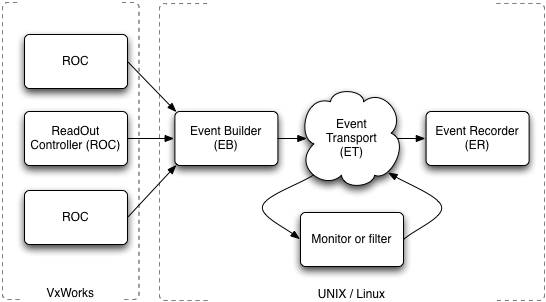
\includegraphics[width=1.0\columnwidth,keepaspectratio]{img/coda_diagram.png}
	\caption{CODA System Diagram}
	\label{fig:coda_diagram}
\end{figure}


\subsection {Run Control}

The CODA DAQ system includes a run control facility consisting of a back-end run control supervisor and a front-end graphical operator display that connects to the supervisor and controls its operation. The supervisor in turn controls operation of the many CODA components that participate in the run. The latter are defined in run configuration files that the operator chooses at startup. The Run Control Graphic User Interface (see Fig.~\ref{fig:runcontrol1}) presents the operator with a choice of possible actions that depend on the current state of the run. The supervisor translates the operator choice into appropriate commands to the individual components. Alternatively, limited communication with the supervisor can be performed via command-line scripts.
In addition, the supervisor monitors the health and operation of the CODA components and warns the operator or pauses the run if problems are detected.

\begin{figure}[hbt]
	\centering
	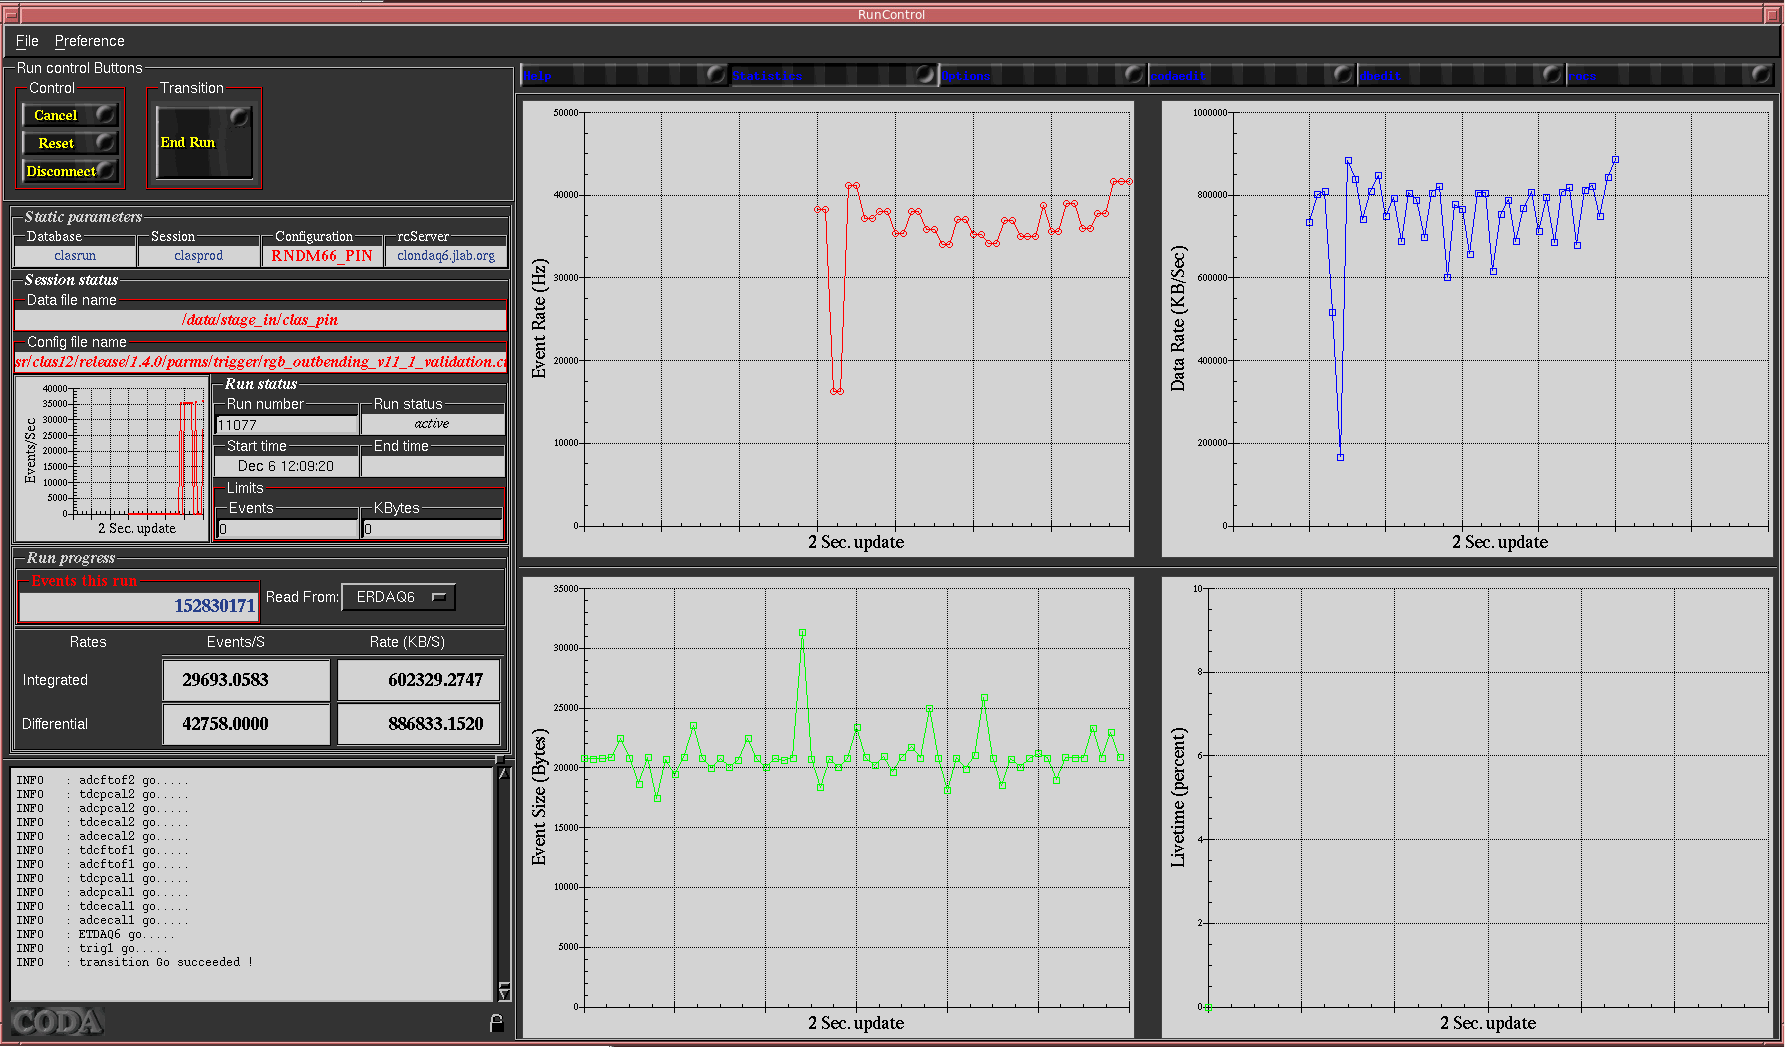
\includegraphics[width=1.0\columnwidth,keepaspectratio]{img/runcontrol1.png}
	\caption{Runcontrol GUI}
	\label{fig:runcontrol1}
\end{figure}


\subsection{Frontend Libraries}

Just an outline ATM

GEFANUC driver:
\begin{itemize}
\item Customized Kernel Driver and Userspace Interface
\item C API provides:
   \begin{itemize}
   \item Setup of VME inbound and outbound windows
      \begin{itemize}
      \item Permanent windows: CRCSR, A16, A24, A32
      \item Map of these windows into userspace
      \end{itemize}
   \item Allocate of Physical Memory for DMA
      \begin{itemize}
      \item Map of this memory into userspace
      \end{itemize}
   \end{itemize}
\end{itemize}

JVME Userspace Driver:
\begin{itemize}
\item C API provides
  \begin{itemize}
  \item common userspace interface to GEFANUC driver and others.
  \item Initialization of kernel driver and default VME windows
  \item Maps VME bridge registers into userspace
    \begin{itemize}
    \item Provides userspace configuration and operation of DMA
    \end{itemize}
  \item Initialization of and access to shared memory mutex for intra-process cooperation during DMA
  \end{itemize}
\end{itemize}

Frontend Libraries
\begin{itemize}
\item C APIs provide
  \begin{itemize}
  \item module register mapping in VME windows to memory structures.
  \item configures modules for readout via
    \begin{itemize}
    \item programmed i/o
    \item Single module DMA
    \item Multiple module DMA
       \begin{itemize}
       \item Token passing (P0/VXS and CBLT) with common A32 address range
       \item Linked List DMA
       \end{itemize}
    \end{itemize}
  \end{itemize}
\end{itemize}



\subsection{Readout Controller}

The Readout Controller (ROC, see Fig.~\ref{fig:roc_diagram}) software component is a program running on the front-end controllers such as the Intel-based VME/VXS crate controllers, VTP trigger boards, or regular Linux servers - essentially any hardware receiving data from the front-end electronics. On the DAQ startup, the ROC main program starts three threads, after that it just controls thread health and communicates with the run control process. Three threads (readout, processing, and network) pass data from one to another, communicating over circular buffers. The typical number of buffers in each circle is 8 and the size of every buffer is 4~MBytes, which defines how long the front-end electronics will be read out before feeling the effect of the back-end busy conditions.

The first thread (readout) receives data from the front-end electronics and places it into the first circular buffer. That thread can run in pooling mode which occupies an entire CPU core, or in interrupt mode. The CLAS12 readout primarely employs pooling mode, which has adequate performance on multi-core controllers. The second thread (processing) reads data from the first circular buffer and performs all needed data processing, in particular it performs the so-called disentangling and data sanity checks. The results are placed into the second circular buffer. That component can create its own threads to increase processing power. The third thread (network) reads data from the second circular buffer and sends it over the network to the Event Builder.

The first and second threads have a user part that is compiled separately and downloaded dynamically, which allows users to develop experiment-dependent code without recompiling the CODA framework.

\begin{figure}[hbt]
	\centering
	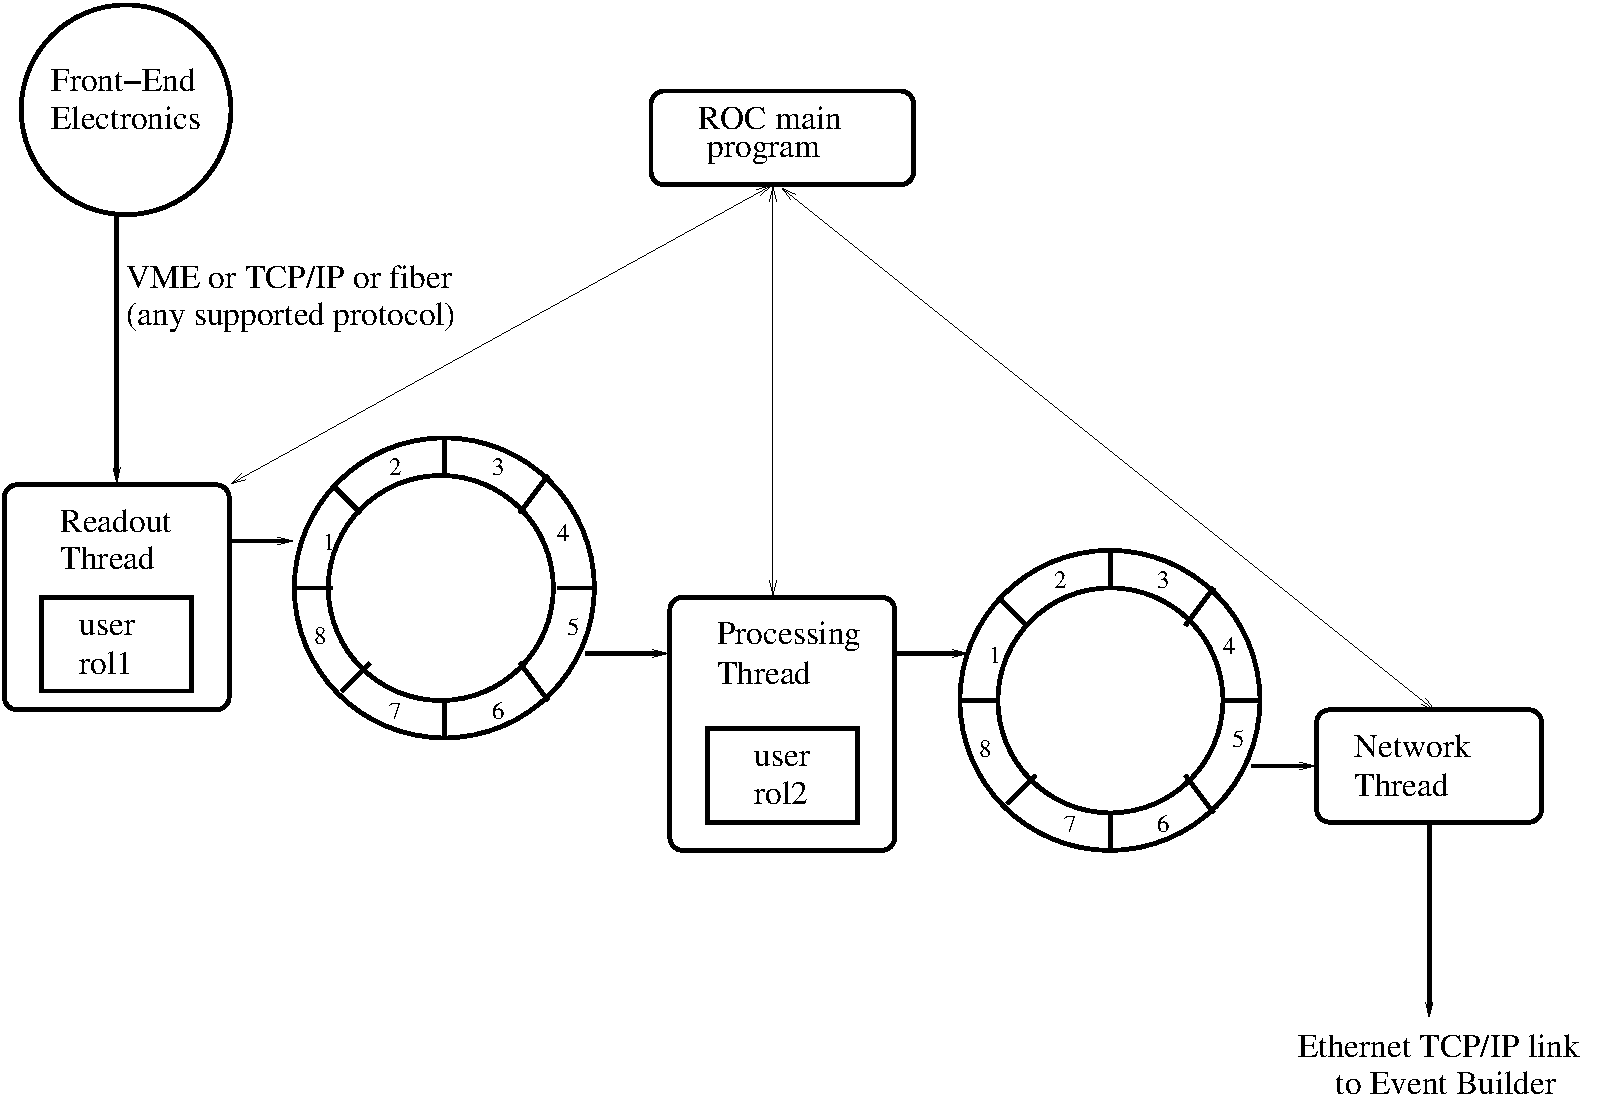
\includegraphics[width=1.0\columnwidth,keepaspectratio]{img/roc_diagram.pdf}
	\caption{Readout Controller Diagram}
	\label{fig:roc_diagram}
\end{figure}


\subsection{Event Builder}

The Event Builder (EB, see Fig.~\ref{fig:eb_diagram}) is the program that receives the data fragments from all readout controllers and assembles it into events. The building process is based on event number, event type, and timestamp of the data fragments: for each event all three values have to be identical for all data from all readout controllers. In case of any differences, the DAQ will be stopped and the error reported.

The Event Builder consists of receiving and building parts. The receiving part contains a set of independent threads, one per readout controller connected to it by TCP protocol. Every thread receives data and places it into an internal buffer. If the buffer becomes full, the thread stops receiving data, effectively propagating the busy condition back to the readout controller. The building part has a number of identical building threads, which take turns by getting data from the receiving part of the internal buffers, building events, and placing them into Event Transfer System.

The total number of threads in the receiving part of the Event Builder in CLAS12 DAQ is currently 118, which therefore represents the number of network connections from the readout controllers. Because of this the DAQ has to run on a powerful server, with many CPU cores, large memory, and a high bandwidth network card. CLAS12 is using a Dell R730 server with 32 cores, 64~GByte memory, and 40~Gbit network card. This server is adequate for the present CLAS12 DAQ requirements.

\begin{figure}[hbt]
	\centering
	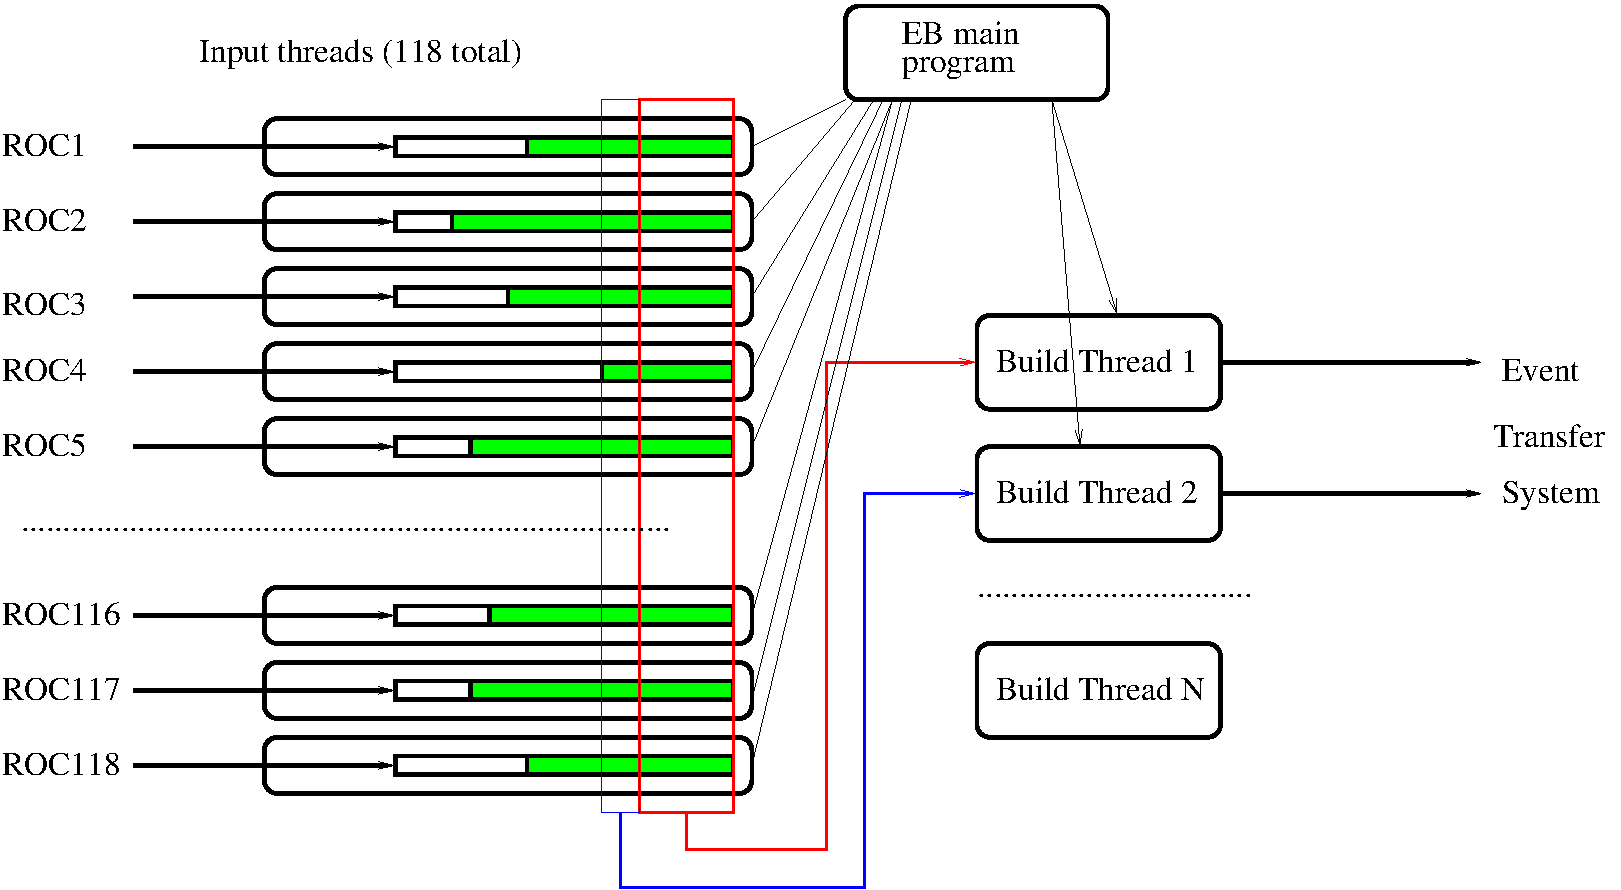
\includegraphics[width=1.0\columnwidth,keepaspectratio]{img/eb_diagram.pdf}
	\caption{Event Builder Diagram}
	\label{fig:eb_diagram}
\end{figure}


\subsection{Event Transfer}

The Event Transfer (ET, see Fig.~\ref{fig:et_diagram}) system provides the user with an efficient method for moving bulk data between processes. The ET was not designed as a messaging system, but it can rather be visualized as data containers moving around a circular railway track. In this metaphor, a producer of data (Event Builder) requests an empty container, fills it with data, tags it with metadata describing the contents, and places it at the start of the track. Stations along the track are assigned algorithms for testing the metadata and selecting the containers of interest. The user has the option of making a station blocking or non-blocking. A container stopped at a blocking station holds up all of the other containers behind it on the track. A data consumer attached to the station processes the data in the container and has the option of either putting the container back on the track, where it proceeds to the next station, or returning the container to the station at the start of the track, effectively discarding the data. In the simple example diagram shown in Fig.~\ref{fig:et_diagram}, a data monitoring consumer attaches to a non-blocking station that samples the data of interest. The Event Recorder attaches to a blocking station and records the content of every container to disk. The container is then returned to the start of the track.

Using these simple concepts, complicated data pathways can be constructed. The ET package supports remote consumers connecting to stations over the network, allowing load sharing between multiple machines. 

\begin{figure}[hbt]
	\centering
	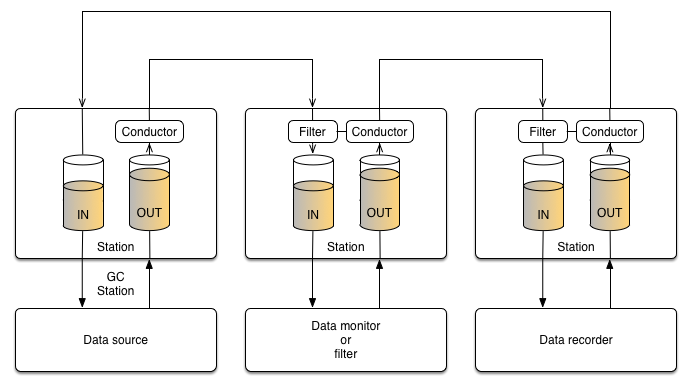
\includegraphics[width=1.0\columnwidth,keepaspectratio]{img/et_diagram.png}
	\caption{Event Transfer System Diagram}
	\label{fig:et_diagram}
\end{figure}

\subsection{Event Recorder}

The Event Recorder (ER, see Fig.~\ref{fig:er_diagram}) is the program that receives data from the ET system and records the data files onto disk. The ER can write data in one or several files in parallel (so-called multi-stream mode). If multi-stream mode is used, the event order is preserved, but it requires the allocated memory size to be bigger than the number of streams multiplied by the file size.

The ER structure in multi-stream mode is shown in Fig.~\ref{fig:er_diagram}. The distribution thread receives data from the Event Transfer system, searches for the free writing thread, and grabs its semaphore. It starts filling up the buffer of the thread with data until it becomes full. After that it signals the writing thread to start writing the entire buffer to the specified output file name. The writing thread marks itself ``busy'' and writes data to the file, and after that, it becomes ``free'' again. While the writing process is in progress, the distribution thread grabs another free writing thread and the process repeats. The writing performance of the ER can be increased by increasing the number of writing threads.

\begin{figure}[hbt]
	\centering
	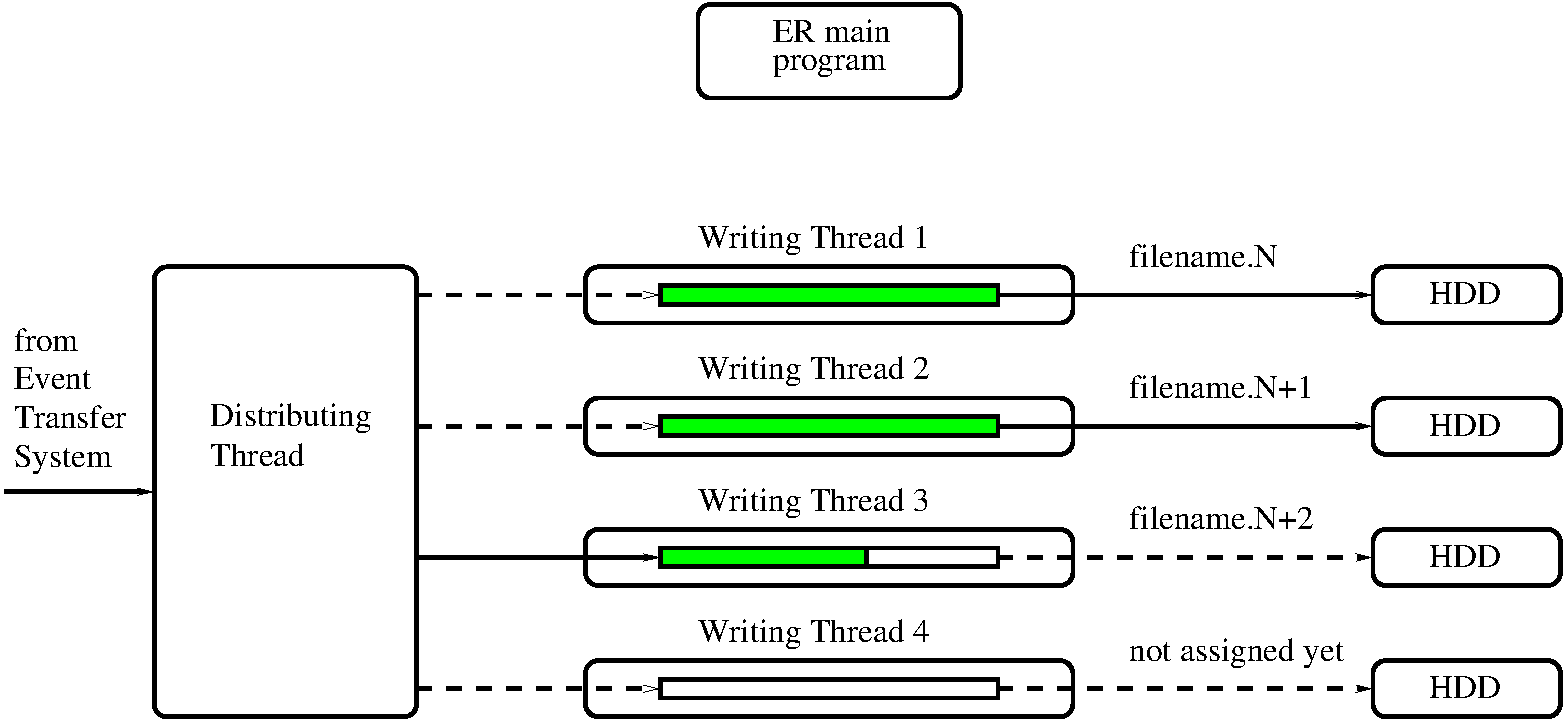
\includegraphics[width=1.0\columnwidth,keepaspectratio]{img/er_diagram.pdf}
	\caption{Event Recorder Diagram}
	\label{fig:er_diagram}
\end{figure}


\subsection{Messaging System (ActiveMQ)}

The messaging system in the CLAS12 DAQ is based on the ActiveMQ library and its C++ extension. Two ActiveMQ servers are used to route all communiations. The number of connections to ActiveMQ is several hundred, and the number of messages sent every second is several tens of thousands, with data volumes of a few tens of MBytes per second. The messaging system is used in particular to monitor and control the DAQ components, in addition to the Run Control process.


\subsection{Runtime Database (RCDB)}

A JLab-designed MYSQL-based Runtime Database (RCDB) is used to store the run parameters and statistics. It has web interface (see Fig.\ref{}) and provides an interface to various languages including C++ and Java.


\subsection{Online Data Monitoring}

The CLAS12 online data monitoring is the set of programs attached to Event Transfer System and processing data in real time. One of such program's output is shown on Fig.\ref{}.


\subsection{ROOT for DAQ (FT)}

A ROOT-based system was developed to display integrated quantities from the CLAS Trigger system in the form of 1D
and 2D histograms. The system is made by three different applications: a histogram sender running on each VTP, a
histogram receiver running on a DAQ server, and a user-configurable GUI client. Each histogram sender application
defines a set of 1D and 2D histograms to report trigger data specific to the CLAS12 subsystem handled by the VTP it is
running on. Histograms are refreshed at a fixed rate and streamed to the DAQ server in the form of JavaScript Object
Notation (JSON) messages, exploiting the previously described ActiveMQ infrastructure. Each message contains: the
histogram name, the number of bins, and a data array with the number of counts in each bin. The message receiver
application is responsible for decoding these messages, and of creating ROOT histograms from them. Finally, the client
application displays ROOT histograms to the user through a customizable GUI.

The GUI is composed of a programmable number of independent frames, with different histograms in each of them.
Typically, each frame contains histograms related to the same CLAS12 subsystem. The GUI structure is specified through
a configuration file passed as a command-line option when running the client. Communication between the message
receiver/ROOT histogram produced application and the user client is handled through the ROOT TSocket mechanism.
Figure~\ref{fig:plot_andrea} shows a GUI reporting histograms from the Forward Tagger system~\cite{ft-ref}: two
2D histograms showing the distribution of electromagnetic cluster hits in the Forward Tagger Calorimeter, and two
1D histograms showing the electromagnetic cluster energy distribution. The right (left) column reports histograms for
electromagnetic clusters  with (without) a matching hit in the Forward Tagger Hodoscope.

\begin{figure}[t]
	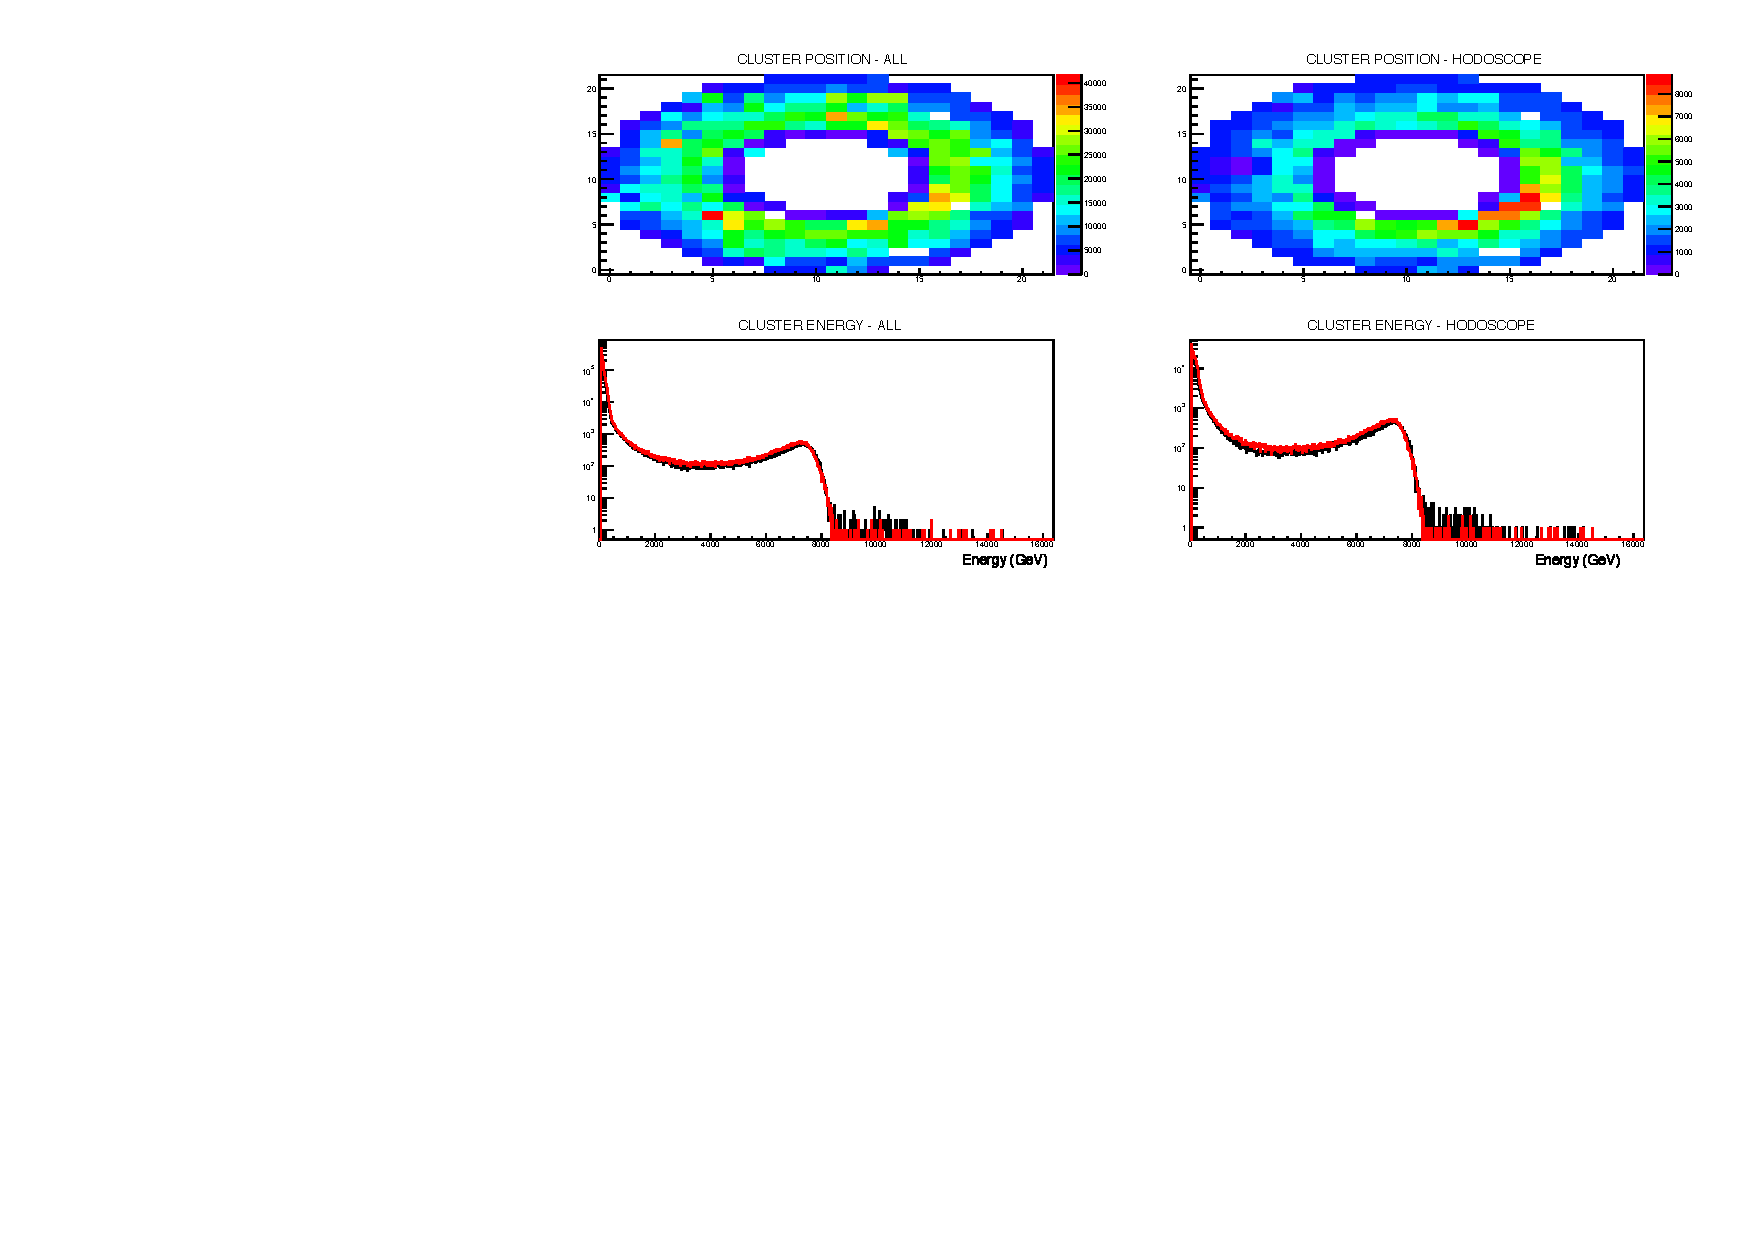
\includegraphics[width=1.0\columnwidth]{img/plotAndrea.pdf}
	\caption{Example of a ROOT-based GUI to monitor trigger data for the specific case of the Forward Tagger
        detector~\cite{ft-ref}. The top histograms report the distribution of electromagnetic cluster hit positions, while
        the bottom histograms report the electromagnetic cluster energy distribution. The right (left) column reports
        histograms for electromagnetic clusters  with (without) a matching hit in the Forward Tagger Hodoscope.}
	\label{fig:plot_andrea}
\end{figure}



\subsection{CLAS Event Display}

The CLAS12 Event Display (CED) is a full-function graphical application that displays on-line (and off-line) events using various representations of CLAS12 called views. The views are independent windows that the user can pan, zoom, scroll, etc. Some of the views are geometrically faithful, and some are designed for maximal information content as opposed to realism. The primary purpose and utility of CED, when used on-line as part of the DAQ system, is for additional data monitoring. While running, CED will display an event from the live stream at a selectable rate, typically one every two seconds. A quick glance at CED will confirm, for example, that there are data in the drift chambers that appear to form tracks. In this way it serves as an early warning of problems with detectors and/or the data stream. It is also possible to operate CED in a mode where it creates graphical histograms or occupancy overlays. A typical view from CED is shown in Fig.~\ref{fig:ced}.

\begin{figure}[hbt]
	\centering
	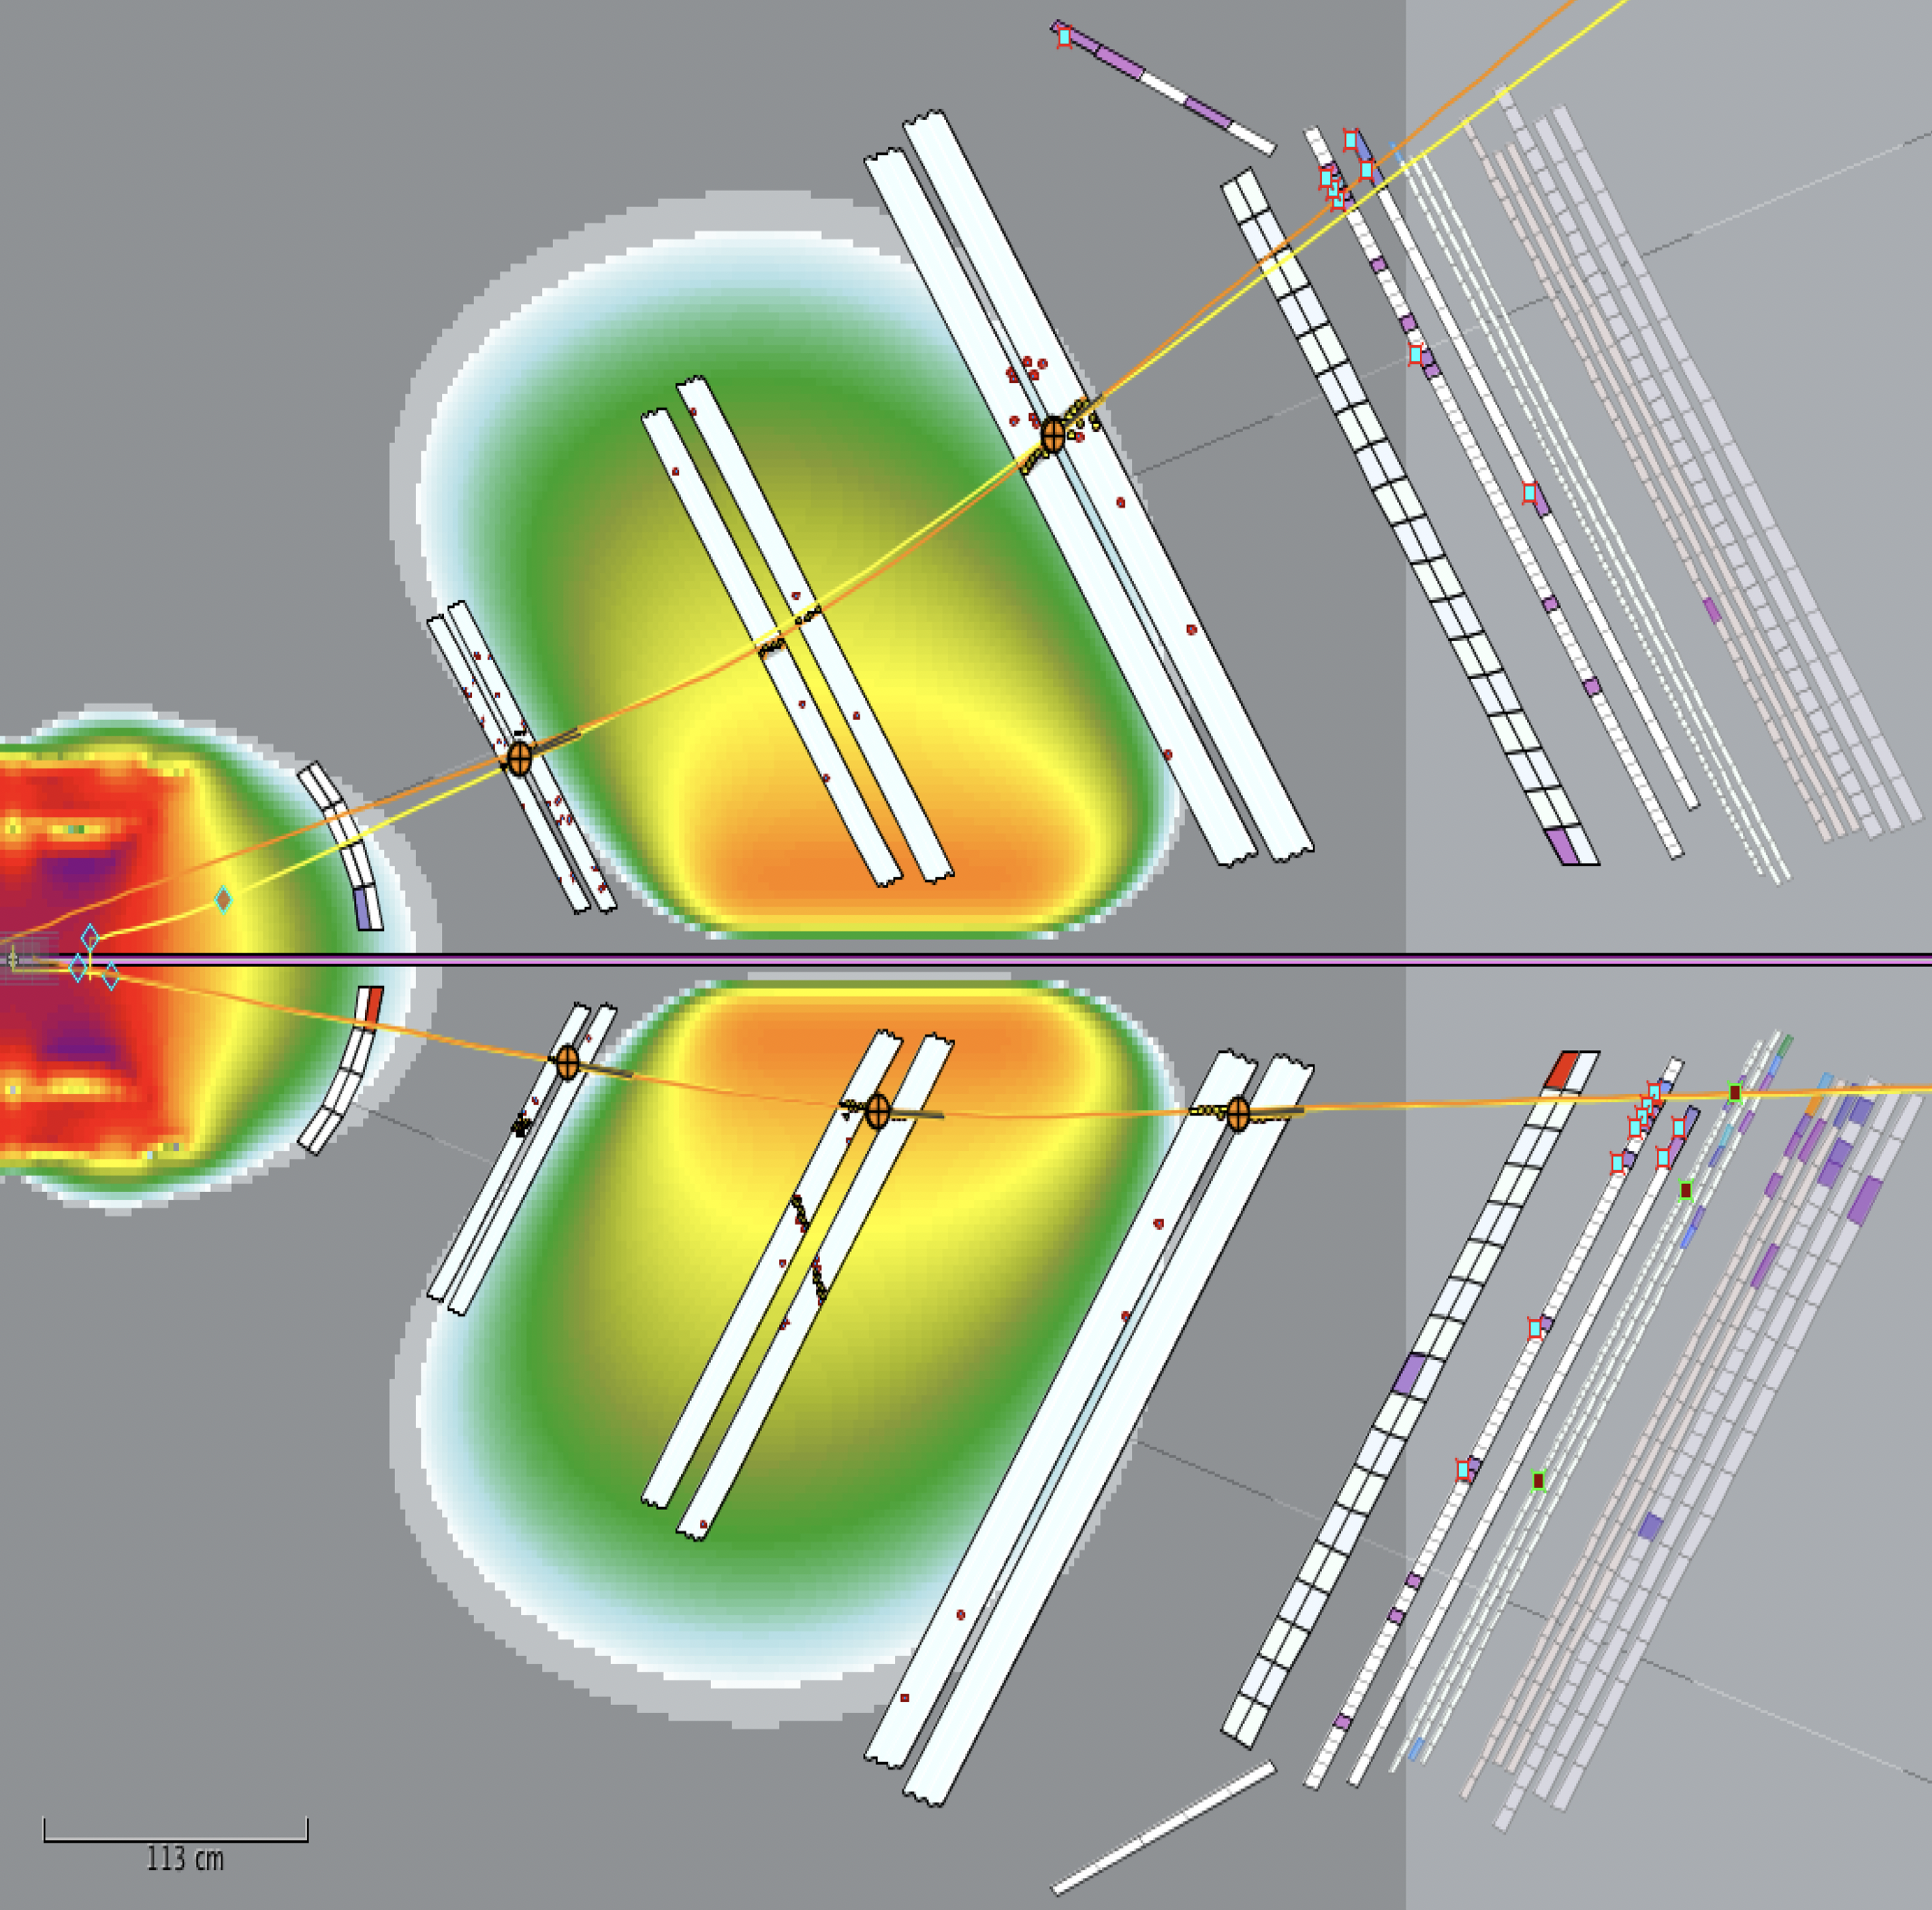
\includegraphics[width=1.0\columnwidth,keepaspectratio]{img/ced.png}
	\caption{CED Event Example}
	\label{fig:ced}
\end{figure}
